\section{Conceptual Overview}
In this section we present a conceptual overview of the subjects of this
study--Workflows and Scientific Workflow Environments.

\subsection{Workflow}
Figure~\ref{fig:wf} shows a typical workflow in the form of a Directed Acyclic
Graph (DAG). Execution typically begins with the input data being provided to
the first task and ends at the results being delivered at the end of the last
task. Tasks are represented by boxes and data/control flow between the task is
represented as arrows. Note that in cases where tasks are connected with pure
control flow, it can be simulated by passing token data between tasks.

For the purpose of this text, we define a workflow as a specification of
computation with at least two discrete tasks either forming distinct
computational stages or running for two or more distinct datasets as
parameters. Consequently, a one-off task or running a task for a single copy of
data is \emph{not} a workflow.

For the rest of this paper, we will use the above definition of a workflow.
%

\begin{figure}[htb]
\begin{center}
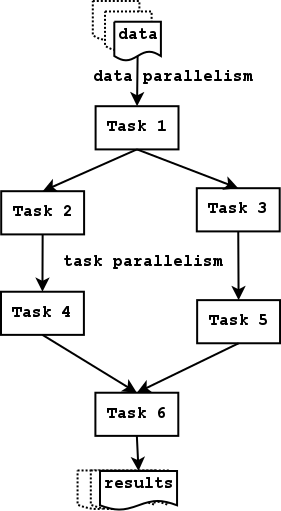
\includegraphics[width=4cm]{figures/workflow}
\caption{A typical workflow depicted as a Directed Acyclic Graph (DAG) of tasks coordinated by data or control flow and illustrating data and task parallelism}
\label{fig:wf}
\end{center}
\end{figure}
%

\subsection{Architecture}
Figure~\ref{fig:wfms} shows a high-level architecture of a generic SWE. It shows key
components and their interaction in an SWE. These components are the focus of
interest for the present work. A \textit{user interface} interacts with the
\textit{workflow engine} using commands and messages on the inside while with
user on the outside. The \textit{workflow language} becomes an intermediate
representation for communication between user interface and the
\textit{workflow engine}. The workflow engine acts as a compiler/interpreter
and a high-level scheduler for the processors and interfaces with the
underlying \textit{distributed resources}. It resolves data dependencies and
optimizes the flow at runtime and monitors the workflow progress and collects
the intermediate and final results.

%
\begin{figure}[htb]
\begin{center}
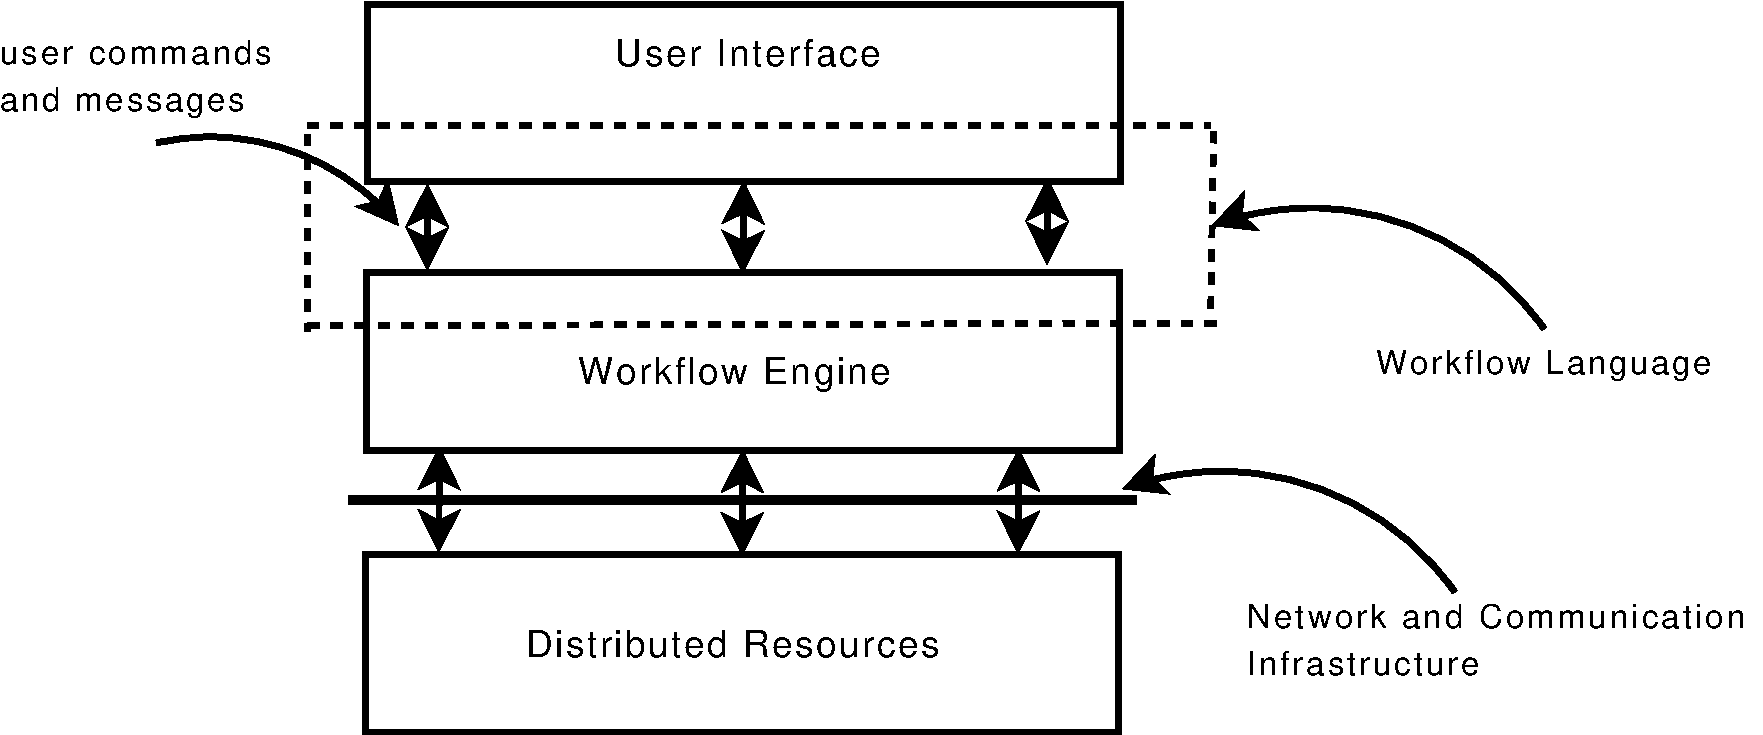
\includegraphics[width=\linewidth]{figures/workflow_interfaces_and_language}
\caption{A generic SWE scheme showing the relationship and interaction among important components}
\label{fig:wfms}
\end{center}
\end{figure}
%
SWEs are used as tools to benefit from the underlying large-scale computing
infrastructure such as clusters, supercomputers, clouds, and grids. Such
environments are in use today for production level work in different scientific
domains worldwide. They do the basic task of linking inter-related processors
of a multi-staged scientific computation. However, they differ in the features
they provide based upon the scientific domain or user community they offer
service for, and the computational model they follow. Often, one of the main
reasons for such difference is the specialized components and requirements for
a particular domain. Owing to this fact, a given workflow system dominates a
particular area of science (eg. astronomy, biology, etc.). Nonetheless, there
exist a plethora of SWEs suitable for general purpose workflow style
computations.

DAGs are by far, the most popular abstraction of the way workflows are
perceived and visualized. The MA DAG~\cite{caron-desprez:2005}, engine is one
example of a DAG generator engine. MA DAG has evolved from a regular DAG
generator to a more abstract DAG generator laced with control structures. MA
DAG benefits from the workflow scheduling mechanisms included in the
middleware. Due to the impossibility to produce complete DAGs owing to the
presence of control structures such as conditionals and loops, MA DAG generate
partial DAGs greedily: a sub-DAG, as complete as possible, is produced as soon
as possible. Despite the presence of many different approaches to workflow
systems, new requirements continue to pose workflow challenges. Some of the
current challenges facing SWEs are:

\begin{enumerate}
\item \textbf{Multisite execution.} Interfacing to existing computation and
storate infrastructure is not trivial, not to mention the new and
unforeseen access and compute modes. SWEs are yet to formulate a
generalized interface towards the major platforms such that they will
run on them out of the box.

\item \textbf{Manysite execution.} Even if a SWE has interfaces built for
more than one infrastructure, it is hard to optimally schedule large
workflows to many remote sites simultaneously. The problem of limited
control over remote sites and distributing interdependent data and
tasks makes it non-trivial to efficiently load-balance work among them.

\item \textbf{Expressivity.} Workflow languages have evolved over the years
with reasonable expressivity being supported. However, they are often
compared with those of the traditional programming languages. As of
current state of the art, the workflow languages expressivity still
have to catch up to the richness of programming languages across
different generations such as C and python.  The community is yet to
realize a truly generic workflow language that can express a wide
variety of flow patterns encountered in scientific domains.

\item \textbf{Interoperability.} Interoperable workflows will benefit to a
broad audience of users. Many efforts at this are made in the recent
past, such as by the consurtium projects and by individual players.
However, a truly interoperable set of standards for workflows are yet
to emerge.
\end{enumerate}
